%%%%%%%%%%%%%%%%%%%%%%%%%%%%%%%%%%%%%%%%%
% Focus Beamer Presentation
% LaTeX Template
% Version 1.0 (8/8/18)
%
% This template has been downloaded from:
% http://www.LaTeXTemplates.com
%
% Original author:
% Pasquale Africa (https://github.com/elauksap/focus-beamertheme) with modifications by 
% Vel (vel@LaTeXTemplates.com)
%
% Template license:
% GNU GPL v3.0 License
%
% Important note:
% The bibliography/references need to be compiled with bibtex.
%
%%%%%%%%%%%%%%%%%%%%%%%%%%%%%%%%%%%%%%%%%

%----------------------------------------------------------------------------------------
%	PACKAGES AND OTHER DOCUMENT CONFIGURATIONS
%----------------------------------------------------------------------------------------

\documentclass{beamer}

\usetheme{Focus} % Use the Focus theme supplied with the template
% Add option [numbering=none] to disable the footer progress bar
% Add option [numbering=fullbar] to show the footer progress bar as always full with a slide count

% Uncomment to enable the ice-blue theme
\definecolor{main}{RGB}{92, 138, 168}
\definecolor{background}{RGB}{240, 247, 255}


%------------------------------------------------

\usepackage{booktabs} % Required for better table rules
\usepackage{hyperref}
\usepackage{graphicx,subfigure}
\usepackage{animate}
\usepackage{textcomp}
%----------------------------------------------------------------------------------------
%	 TITLE SLIDE
%----------------------------------------------------------------------------------------

\title{Interfacing EMCCD Camera used in Ion Trap experiments}



\author{Yudi Wu}

\titlegraphic{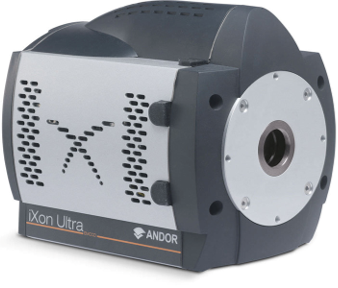
\includegraphics[scale=0.27]{Figures/iXon-Ultra-897.png}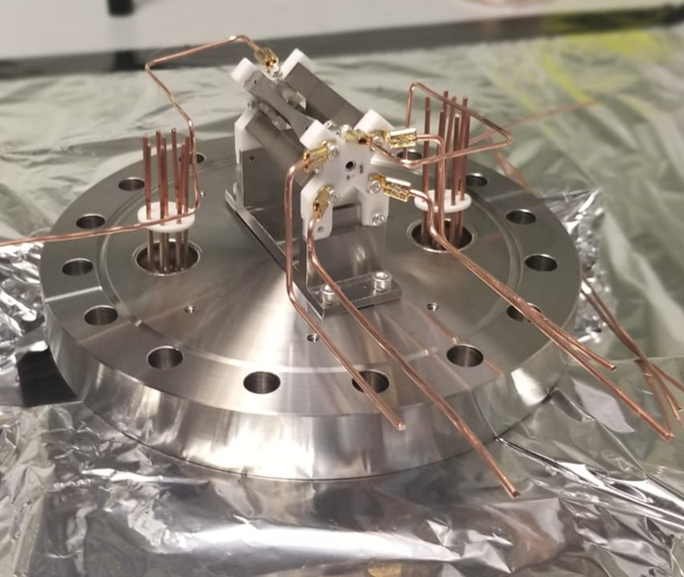
\includegraphics[scale=0.18]{Figures/ion_trap_photo.png}} % Optional title page image, comment this line to remove it

\institute{Imperial College London}

\date{16/07/2019}

%------------------------------------------------

\begin{document}

%------------------------------------------------

\begin{frame}
		\maketitle % Automatically created using the information in the commands above
\begin{picture}(0,0) 
    % \put{} defines the position of the frame
    \put(240,240){\makebox(20,40)[bl]{
    
\includegraphics[scale=0.5]{Figures/IC_logo.png}
    }}%
  \end{picture}%
\end{frame}


%------------------------------------------------
\begin{frame}
\frametitle{{Overview}}
\tableofcontents[]
\end{frame}


\AtBeginSection[]
{
  \begin{frame}<beamer>
    \tableofcontents[currentsection]
  \end{frame}
}


%------------------------------------------------
\section{Iontraps and EMCCD Cameras}
\begin{frame}{Ion traps}
\frametitle{}
\begin{itemize}
\item Ion trap: e.g. Penning or Paul trap, used to levitate small clouds of ions, or a single atomic ion, in free
space, inside a vacuum chamber.
\bigskip
\item Typically lasers used to manipulate the ions and an imaging system to detect the ion's fluorescence
\end{itemize}
\vspace{0.3cm}
\centering
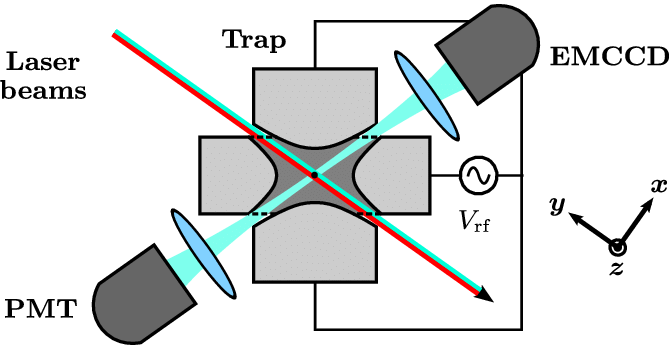
\includegraphics[height=3.4 cm]{Figures/Paul_trap_schematics.png}
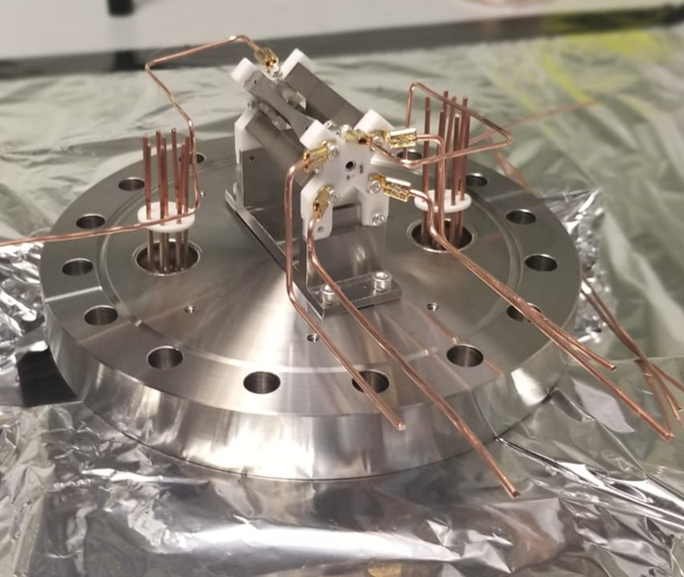
\includegraphics[height=3.4 cm]{Figures/ion_trap_photo.png}
\end{frame}

%------------------------------------------------
\begin{frame}{EMCCD Cameras}

\begin{itemize}
\item Charged Coupled Device (CCD): silicon based semiconductor chip, captures light, converts the photons to digital data in the form of electrons
\bigskip
\item Electron Multiplying CCD (EMCCD):  identical structure to conventional CCDs BUT more sensitive and capable of single photo detection (e.g. fluorescence of single ions)
\bigskip
\item EMCCDs widely used in ion trap experiments
\end{itemize}

\centering
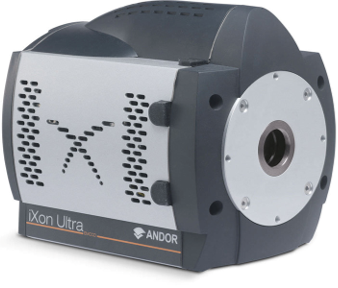
\includegraphics[scale=0.38]{Figures/iXon-Ultra-897.png}

\end{frame}

%------------------------------------------------

\begin{frame}{EMCCD Cameras}

\begin{columns}
          \column{0.45\linewidth}
             \centering
             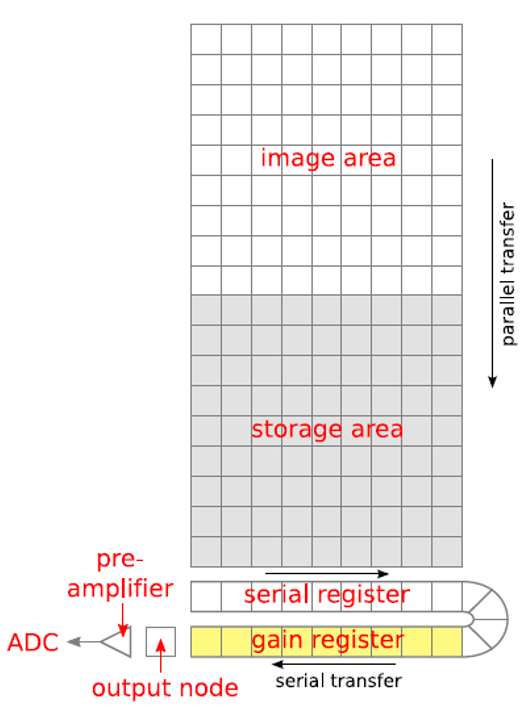
\includegraphics[width=4.3 cm]{Figures/EMCCD_Structure.PNG}
           \column{0.62\linewidth}
              \begin{itemize}
\item Shift register extended with Gain register => significantly improves low light detection
\bigskip
\item Possible to read out only a part of the detector array
\end{itemize}
         \end{columns} 


\end{frame}

%------------------------------------------------

\section{My Tasks}

\begin{frame}{My Tasks}
\frametitle{}
\begin{itemize}
\item Write a Python 3 program around existing library to interface our Andor iXon Ultra EMCCD camera
	\begin{itemize}
	\item Commercial software fine for general imaging, but Python program can be tailored to experimental requirements
	\end{itemize}
\bigskip
\item Find a method of distinguishing between a bright and a dark ion
\bigskip
\item Find optimal parameter settings to obtain best image in shortest exposure time
\end{itemize}


\end{frame}

%------------------------------------------------

\section{Current Progress}
\begin{frame}{The Program}
\frametitle{}

\begin{itemize}
\item Two separate programs: the EMCCD camera control program and the image loading program
\bigskip
\item A Dynamic Link Library (DLL) containing various functions of the camera used by the program to control the camera
\bigskip
\item Both programs are object oriented and have a graphical user interface (GUI) created using QT Creator software
\bigskip
\item UI file from QT Creator converted to Python script with PyQt5 module => no need to write GUI in Python from scratch!
\end{itemize} 


\end{frame}

%------------------------------------------------
\begin{frame}{The Program (cont.)}

\begin{figure}
\begin{center}
\subfigure[Camera control program architechture]{\label{fig:a}
\includegraphics[scale=0.3]{Figures/cam_flow_chart.png}}
\subfigure[Image loading program architechture]{\label{fig:b}
\includegraphics[scale=0.3]{Figures/img_load_flow_chart.png}}
\end{center}
\end{figure}



\end{frame}

%------------------------------------------------
\begin{frame}{Camera Control Program}

\begin{figure}
\centering
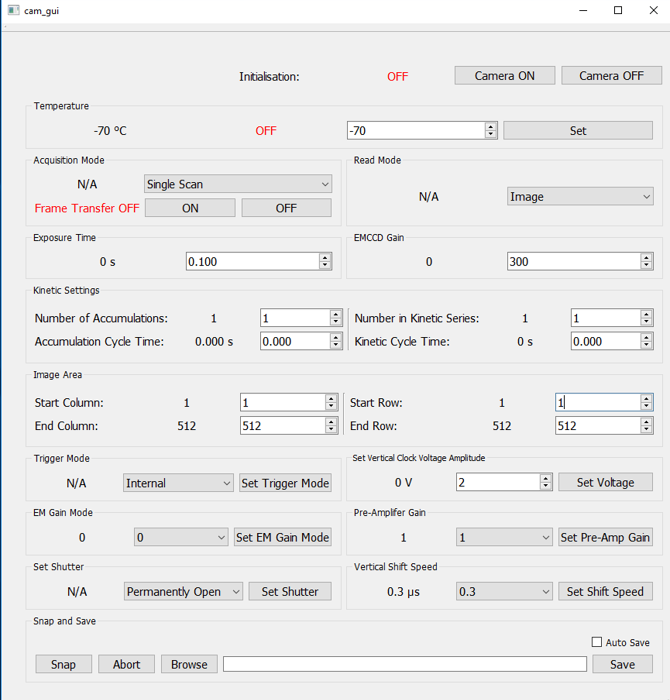
\includegraphics[scale=0.32]{Figures/cam_program.PNG}
\end{figure}


\end{frame}

%------------------------------------------------
\begin{frame}{Image Loading Program}


\begin{center}
	\animategraphics[width=\textwidth,autoplay,loop]{2.5}{Figures/pic_load/pl_frame_}{01}{36}
\end{center}

\end{frame}

%------------------------------------------------
\begin{frame}{Investigating Camera Properties}

\begin{itemize}
\item The camera control program was first tested with noise readings and compared with commercial software to ensure the python program is working as expected
\bigskip
\item The affect of the Exposure time and EMCCD gain on the mean noise reading per pixel were tested

\end{itemize}



\end{frame}

%------------------------------------------------
\begin{frame}{ Exposure Time and EMCCD Gain}


\begin{figure}
\centering     
\subfigure{\label{fig:a}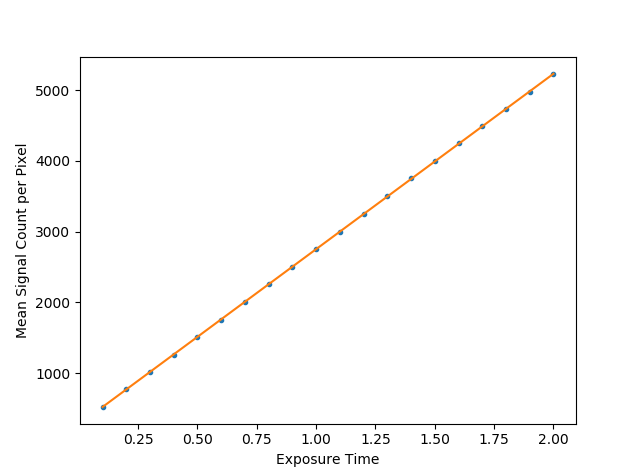
\includegraphics[scale = 0.24]{Figures/Noise_Python.png}}
\subfigure{\label{fig:b}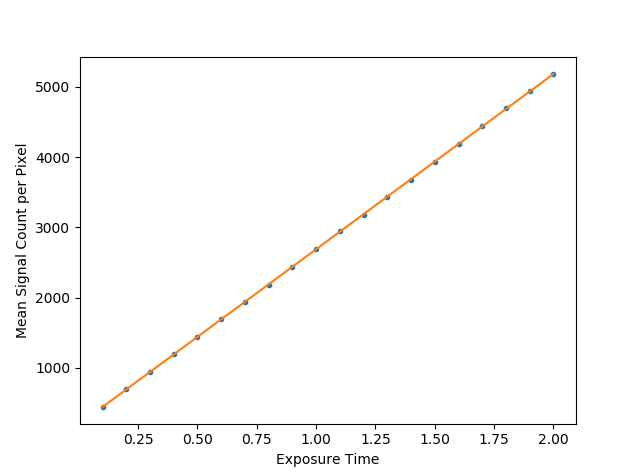
\includegraphics[scale = 0.24]{Figures/Noise_Commercial.png}}
\renewcommand{\thesubfigure}{(a)} 
\subfigure[Python Program]{\label{fig:c}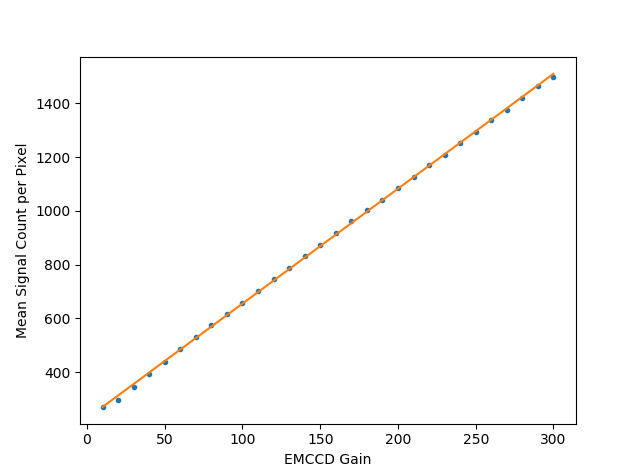
\includegraphics[scale = 0.24]{Figures/Gain_Python.png}}     
\renewcommand{\thesubfigure}{(b)}     
\subfigure[Commercial Software]{\label{fig:d}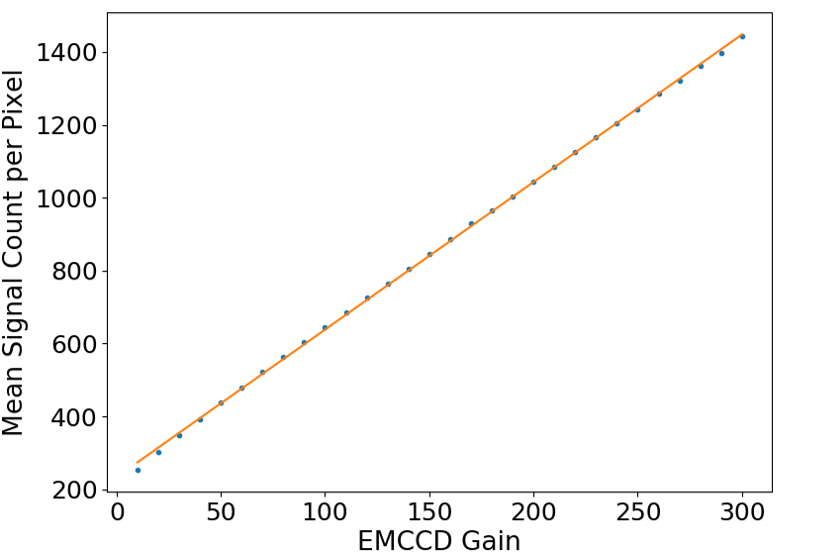
\includegraphics[scale = 0.24]{Figures/Gain_Commercial.png}}
%\caption{ Mean Signal Count vs. Exposure time comparison between a) Python and b) Commercial software. Mean Signal Count vs. EMCCD Gain comparison between c) Python and d) Commercial software}
\end{figure}

\end{frame}

%------------------------------------------------

\begin{frame}{Images of Single Ion at Different Exposure Times}

\begin{itemize}
\item Each Pixel of 16 \textmu m x 16 \textmu m, magnification of imaging system: x10
\bigskip
\item diameter of ion image $\sim$ 6 pixels => diameter of ion fluorescence $\sim$ 9.6 \textmu m

\end{itemize}


\begin{figure}
\centering
\renewcommand{\thesubfigure}{(a)}     
\subfigure[5 Second Exposure]{\label{fig:a}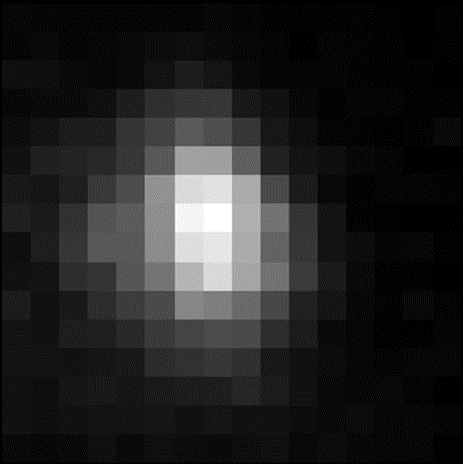
\includegraphics[width=36mm]{Figures/5_sec_exposure.png}}
\renewcommand{\thesubfigure}{(b)}     
\subfigure[2 Second Exposure]{\label{fig:b}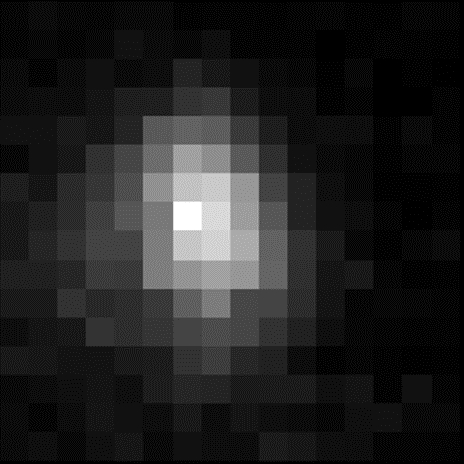
\includegraphics[width=36mm]{Figures/2_sec_exposure.png}}
\renewcommand{\thesubfigure}{(c)}     
\subfigure[1 Second Exposure]{\label{fig:c}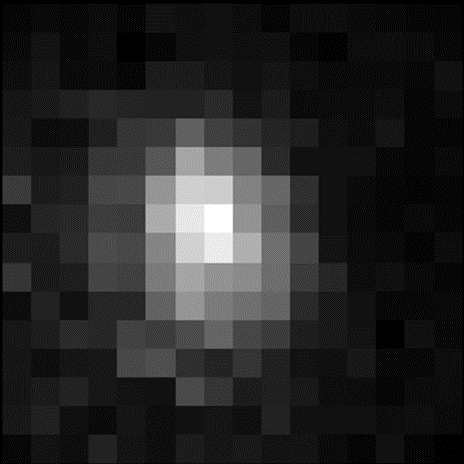
\includegraphics[width=36mm]{Figures/1_sec_exposure.png}}
\end{figure}


\end{frame}



%------------------------------------------------
\begin{frame}{Images of Single Ion at Different Exposure Times (cont.)}



\begin{figure}
\centering
\renewcommand{\thesubfigure}{(d)}     
\subfigure[0.7 Second Exposure]{\label{fig:d}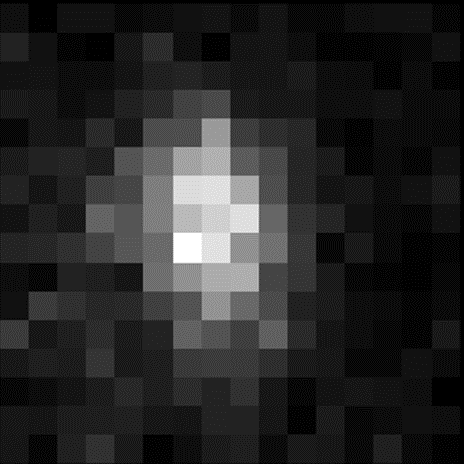
\includegraphics[width=36mm]{Figures/700ms_exposure.png}}
\renewcommand{\thesubfigure}{(e)}     
\subfigure[0.4 Second Exposure]{\label{fig:e}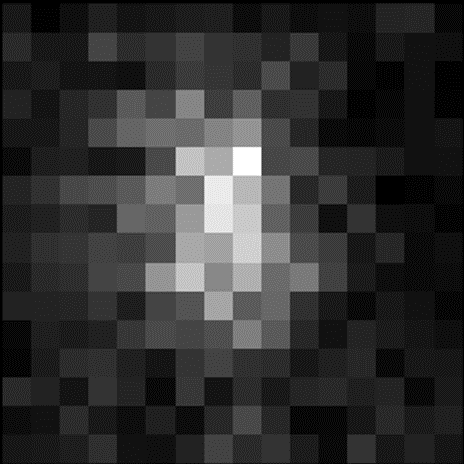
\includegraphics[width=36mm]{Figures/400ms_exposure.png}}
\renewcommand{\thesubfigure}{f)}     
\subfigure[0.1 Second Exposure]{\label{fig:f}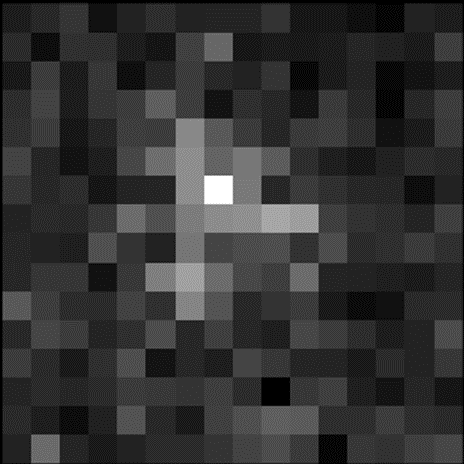
\includegraphics[width=36mm]{Figures/100ms_exposure.png}}
\end{figure}


\end{frame}



%------------------------------------------------

\section{Next Steps}
\begin{frame}{Next Steps}
\frametitle{}
\begin{itemize}
\item Investigate the minimum exposure required for a bright ion to be able to be distinguished from a dark ion
\bigskip
\item A bright ion can no longer be distinguished from a dark ion if the distibution (P) of the brignt (B) and dark (D) ion signal counts have a large overlap

\end{itemize}

\begin{figure}
\centering
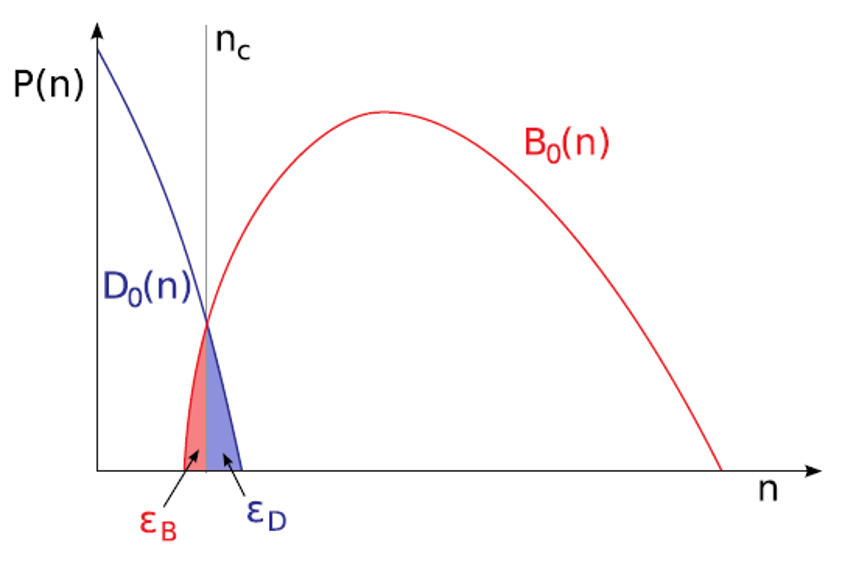
\includegraphics[scale=0.3]{Figures/B_D_graph.png}
\end{figure}

\end{frame}

%------------------------------------------------
\begin{frame}{Future Plans (cont.)}

\begin{itemize}
\item Comparing the differences in quality for image taken when the camera is externally triggered by the experiment and when the camera triggers the experiment and the start of exposure
\bigskip
\item The EMCCD has a 'keep clean' cycle which clears the sensor to ensure it is charge free before the next exposure.
\bigskip
\item Externally triggering the camera may interrupt the 'keep clean' cycle and produce a more noisy image
\bigskip
\item The camera gives off a 'fire signal' during exposure => can be used to trigger the start of the experiment at the end of a 'keep clean' cycle
\end{itemize}


\end{frame}

%------------------------------------------------
\begin{frame}{Conclusion}

\begin{itemize}
\item A Python program with a GUI was created to acquire pictures of fluorescence of single ions and another program was created to view the images and show the vertical and horizontal projections
\bigskip
\item A reliable method/algorithm is required to distinguish bright ions from dark ions at short exposure time
\bigskip
\item Find the camera triggering mode which gives images of highest signal to noise ratio

\end{itemize}


\end{frame}

%------------------------------------------------
\begin{frame}[noframenumbering]

\centering
Thank You for Listening!



\end{frame}


%------------------------------------------------


\end{document}
